\subsection{Hit Finding/Clustering}
After noise reduction we find signal hits and create clusters associated to single tracks. 
Hit is defined as bump over given threshold in a channel. 
Threshold of hit finding is 6 ADC counts, which is about 2.5$\sigma$ from typical data noise level (as shown in Fig~\ref{Fig:afterFFT}) and keeping more than 99\% of Kaon hit finding efficiency in simulation.
% noise level from outside window of PhysicsOct55 (rms~2.49)
ADC count distribution is fitted by Gaussian plus step function to estimate the charge of hit in ADC $\times$ $\mu$s unit.
Fitting $\chi^2 < 3$ and $2.5<$~(time~width~of~hit)~$<8$~$\mu$s are required to remove noise hits further.
After finding all hits in an event, we construct cluster by merging adjacent hits. 
The example of hit finding and clustering using Fig~\ref{Fig:Textbook} event is shown in Fig~\ref{fig:Clustering}, which indicates reasonable hit and cluster findings. 

\begin{figure}[htbp]
 \begin{center}
  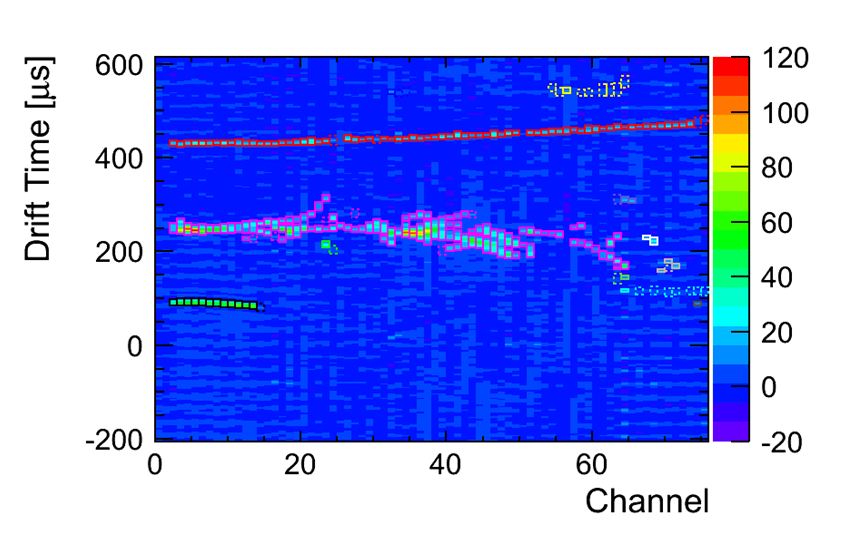
\includegraphics[width=100mm]{fig/clustering.eps}
 \end{center}
 \caption{Example of hit finding and clustering. A colored box corresponds to a hit and colors represent different clusters.}
 \label{fig:Clustering}
\end{figure}

%\begin{itemize}
%\item Plot: Finding efficiency vs threshold (Naganoma): TBU
%\item Plot: Through-going pion data Q vs pion (Tanaka)
%\end{itemize}
